%Table & actions
\subsection{Table}
%~~~~~~~~~~~~~~~~~~~~~~~~~~~~~~~~~~~~~~~~~~~~~~~~~~~~~~~~~~~~
\paragraph{}
La réalisation de la table fut l'un des premiers objectifs cruciaux à atteindre. 

\noindent En effet, requérant un investissement important de temps, la table est essentielle pour avoir une idée visuelle des actions que devront réaliser les robots et donc permettre de tester les prototypes en situation réelle. On peut ajouter également qu'avoir un élément physique terminé donne l'agréable sensation d'être sur le bon chemin et redonne du cœur à l'ouvrage.

\paragraph{}
Sa mise en œuvre fut divisée en plusieurs étapes : 
\begin{itemize}
	\item Achat des matériaux : peinture, bois et vis;
	\item Découpe des planches;
	\item Assemblage;
	\item Peinture;
	\item Tracés des détails : ligne noire, logo, etc..
\end{itemize}

\paragraph{}
La production se déroula sur les premiers mois du projet (octobre à novembre).

\noindent Après la livraison des planches découpées à la fin de la semaine de Toussaint (03/11), l'équipe s'est relayée pour effectuer l'assemblage et la peinture des différents éléments.

\noindent La réalisation de la table ne posa aucun problème majeur hormis un détail : La dimension d'épaisseur requise des planches (20mm) n'est pas une norme belge et ne pouvait être négligée, car elle sert, entre autre, à réaliser les marches de l'escalier. Cela impliqua un délai supplémentaire lors de la commande retardant inévitablement la découpe. Le résultat est visible sur la figure~\ref{img:table}.

\begin{figure}[!ht]
	\centering
	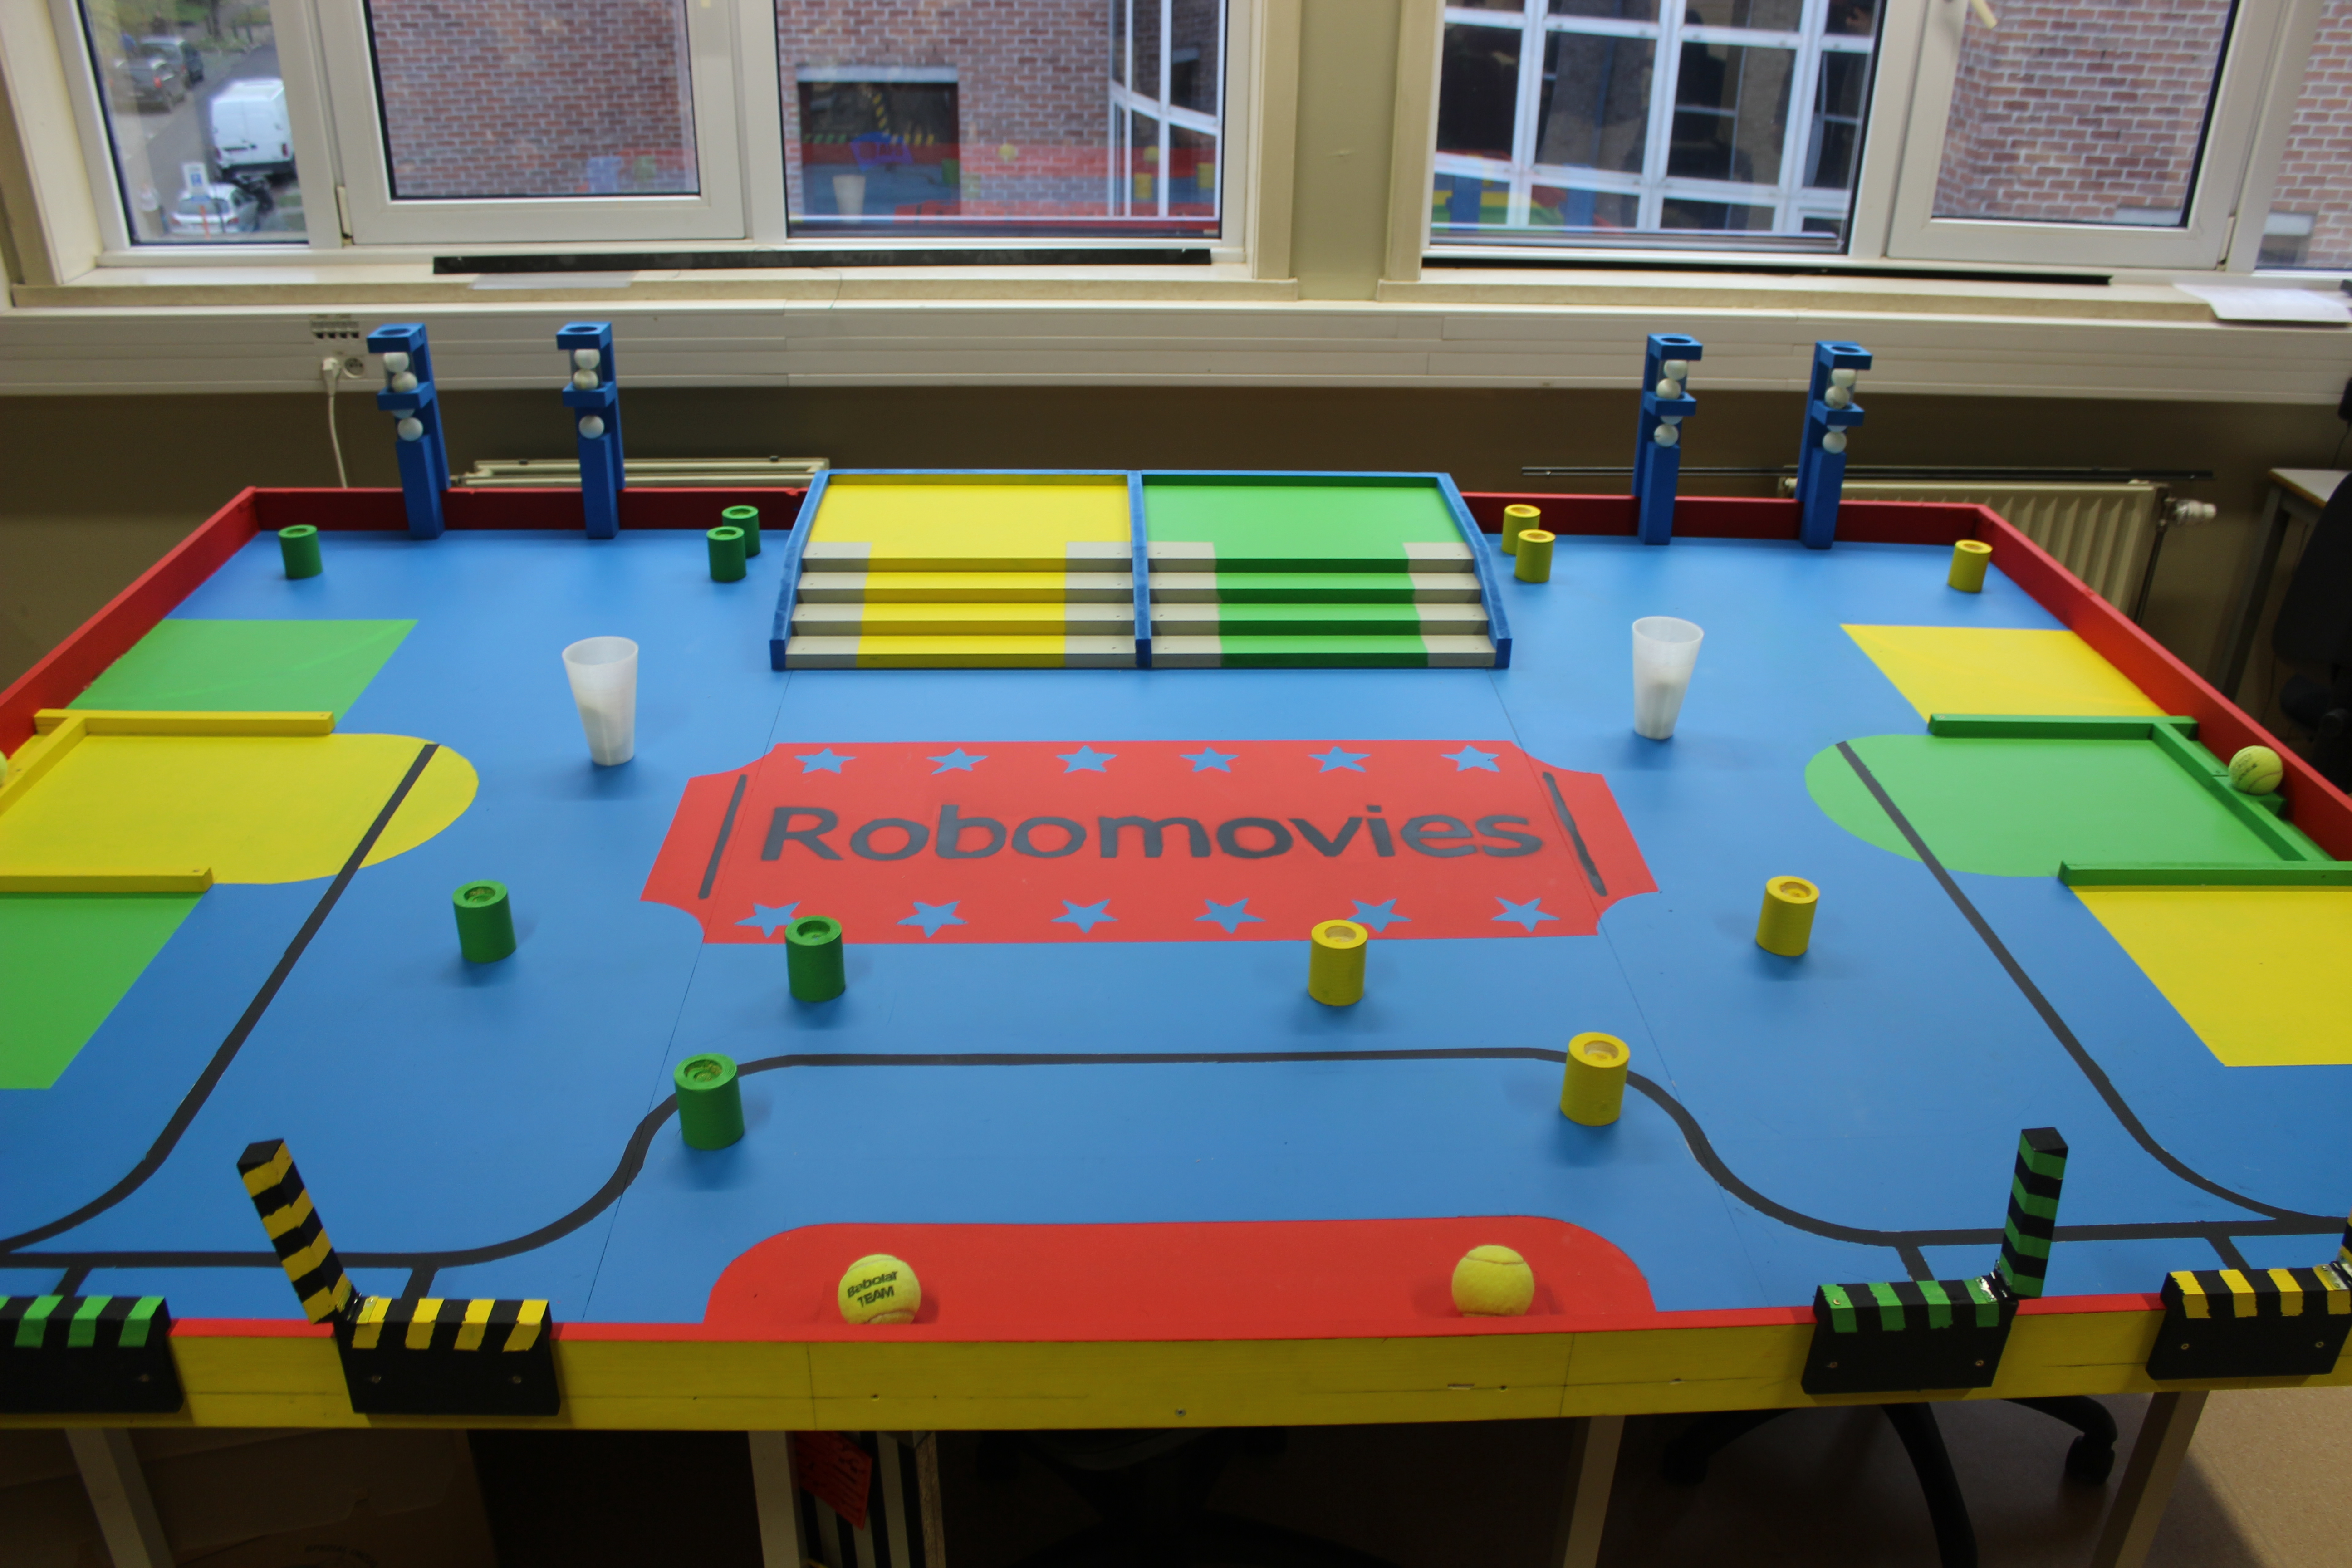
\includegraphics[width=15cm]{Eurobot_Table_1.JPG}
	\caption{Table}
	\label{img:table}
\end{figure}

\subsection{Action des robots}
%~~~~~~~~~~~~~~~~~~~~~~~~~~~~~~~~~~~~~~~~~~~~~~~~~~~~~~~~~~~~
\subsubsection{Introduction}
%~~~~~~~~~~~~~~~~~~~~~~~~~~~~~~~~~~~~~~~~~~~~~~~~~~~~~~~~~~~~
Chaque match est composé de 5 épreuves à réaliser grâce à 1 ou 2 robots indépendants. Aucun contact entre les adversaires n’est autorisé sous peine de malus donc les robots devront être prompts à s’arrêter en cas de rencontre.

\subsubsection{The spotlight}
%~~~~~~~~~~~~~~~~~~~~~~~~~~~~~~~~~~~~~~~~~~~~~~~~~~~~~~~~~~~~
Le robot devra bâtir des spotlights. Pour ce faire, il devra aller récupérer des stands de sa couleur (8 au total) et les amener dans une des zones de construction (1 par équipe + 1 commune).  Ensuite, il suffira d’empiler les stands le plus haut possible et de placer une balle de tennis (4 disponibles, mais communes aux 2 équipes) à son sommet.

\noindent Chaque stand présent dans la zone de construction personnelle rapportera des points mais un seul spotlight peut y être construit. Les autres devront être réalisés dans la zone commune.

\noindent On ne peut en aucun cas interagir avec les stands adverses et un spotlight placé sur la plateforme de la zone commune ne peut être altéré (vol de la balle de tennis) par l’adversaire.

\paragraph{}
Chaque plot rapporte 2 points s’il est correctement placé dans une zone de construction et 3 points bonus par spotlight valide (tour avec balle de tennis).

\subsubsection{The clapperboards}
%~~~~~~~~~~~~~~~~~~~~~~~~~~~~~~~~~~~~~~~~~~~~~~~~~~~~~~~~~~~~
Le robot devra aller fermer les clapperboards correspondant aux couleurs de son équipe qui sont au nombre de 3 (2 proches de sa zone de départ et 1 chez l’adversaire). Il peut se servir de la ligne noire tracée au sol pour se diriger facilement jusqu’aux clapperboards.

\paragraph{}
Cette épreuve rapporte 5 points par clapperboard correctement fermé.

\subsubsection{The popcorn}
%~~~~~~~~~~~~~~~~~~~~~~~~~~~~~~~~~~~~~~~~~~~~~~~~~~~~~~~~~~~~
Le robot devra récolter des popcorns et soit les amener dans sa base et les placer dans la rigole de récupération soit les placer dans un gobelet et l’amener dans une des 3 zones « cinéma » appartenant à son équipe (1 gobelet maximum par zone, le plus rempli sera pris en compte). 

\noindent Les popcorns sont initialement mis dans les gobelets ou dans les machines de distribution. La table proposera 5 verres contenant chacun 4 popcorns et 4 machines avec 5 popcorns.

\noindent Il est nécessaire de savoir que les gobelets placés dans un cinéma peuvent être « volés » par l’équipe adverse.

\paragraph{}
Chaque popcorn présent dans un gobelet placé dans une zone « cinéma » ou placé dans la rigole de la base rapportera 1 point.

\subsubsection{Climbing the red carpet steps}
%~~~~~~~~~~~~~~~~~~~~~~~~~~~~~~~~~~~~~~~~~~~~~~~~~~~~~~~~~~~~
Le robot devra se diriger vers les escaliers situés à l'arrière de la zone de jeu, gravir les marches pour se trouver au sommet à la fin du match.

\paragraph{}
15 points seront attribué en cas de réussite.

\subsubsection{The red carpet}
%~~~~~~~~~~~~~~~~~~~~~~~~~~~~~~~~~~~~~~~~~~~~~~~~~~~~~~~~~~~~
Le robot devra placer de part et d’autre de son escalier un bout de tissu rouge sur les marches de couleurs grises. Pour ce faire, le plus simple sera de monter au sommet et, ensuite, de dérouler le tissu préalablement roulé et mis à bord du robot. 

\paragraph{}
Chaque marche (4 au total x 2) couverte rapportera 2 points et un bonus de 4 points sera offert par volée complètement couverte.

\subsubsection{Bonus/Malus}
%~~~~~~~~~~~~~~~~~~~~~~~~~~~~~~~~~~~~~~~~~~~~~~~~~~~~~~~~~~~~
Toute pénalité impliquera un retrait de 10 points à l'équipe jusqu'à un minimum de 0.
\noindent Il est important se savoir que pour valider un point, le robot ne peut plus avoir d'emprise sur l'objet en question : si en déplacant le robot sur son axe de déplacement principal en impliquant un mouvement de l'objet, celui-ci ne sera pas valide.
\noindent Et, pour finir, 5 points seront attribués à chaque équipe qui n'est pas considérée comme "scratched" : robot présent et fonctionnel.

\subsubsection{Situation Actuelle}
%~~~~~~~~~~~~~~~~~~~~~~~~~~~~~~~~~~~~~~~~~~~~~~~~~~~~~~~~~~~~
Dans notre cas, nous alignerons 2 robots qui s'occuperont chacun de plusieurs tâches distinctes. 

\noindent Le principal s'occupera des 3 premières épreuves : The spotlight, The clapperboards et The popcorn. Tandis que le second s’occupera des escaliers : Climbing the red carpet steps et The red carpet.

\paragraph{}
Pour assurer ces deux dernières opérations, le choix s’est orienté vers l’achat d’un robot à chenille déjà assemblé compatible avec arduino. Nous l’avons choisi notamment pour sa bonne répartition du poids et sa facilité à franchir les marches d’escalier.  

\paragraph{}
Pour le moment, notre attention est dirigée sur The clapperboards et Climbing the red carpet steps qui, en plus de rapporter une bonne quantité de points sans trop de difficulté (3*5 + 15 points), parcoure l'ensemble des fonctionnalités primaires attendues chez nos 2 robots à savoir le déplacement, la détection et la gestion des obstacles, la maitrise de la pince mécanique et l'escalade des marches.

\noindent Pour les autres épreuves, nous n’avons pas encore déterminé l’ordre des actions que le robot effectuera et comment il devra réagir en situation réelle.